%% LyX 2.0.5.1 created this file.  For more info, see http://www.lyx.org/.
%% Do not edit unless you really know what you are doing.
\documentclass[british]{article}
\renewcommand{\familydefault}{\sfdefault}
\usepackage[T1]{fontenc}
\usepackage[utf8]{luainputenc}
\usepackage{listings}
\usepackage{geometry}
\geometry{verbose,tmargin=2cm,bmargin=2cm,lmargin=2cm,rmargin=1.5cm,headheight=2cm}
\usepackage{fancyhdr}
\pagestyle{fancy}
\setcounter{tocdepth}{2}
\setlength{\parskip}{\medskipamount}
\setlength{\parindent}{0pt}
\usepackage{color}
\usepackage{babel}
\usepackage{verbatim}
\usepackage{refstyle}
\usepackage{float}
\usepackage{wrapfig}
\usepackage{units}
\usepackage{amsmath}
\usepackage{amssymb}
\usepackage{fixltx2e}
\usepackage{graphicx}
\usepackage{setspace}
\usepackage[authoryear]{natbib}
\PassOptionsToPackage{normalem}{ulem}
\usepackage{ulem}
\onehalfspacing
\usepackage[unicode=true,pdfusetitle,
 bookmarks=true,bookmarksnumbered=true,bookmarksopen=false,
 breaklinks=false,pdfborder={0 0 0},backref=false,colorlinks=true]
 {hyperref}
\hypersetup{
 linkcolor=blue, bookmarks=false, pdfstartview={FitH},citecolor=Bittersweet}

\makeatletter

%%%%%%%%%%%%%%%%%%%%%%%%%%%%%% LyX specific LaTeX commands.

\AtBeginDocument{\providecommand\secref[1]{\ref{sec:#1}}}
\AtBeginDocument{\providecommand\figref[1]{\ref{fig:#1}}}
\AtBeginDocument{\providecommand\eqref[1]{\ref{eq:#1}}}
\AtBeginDocument{\providecommand\tabref[1]{\ref{tab:#1}}}
%% Because html converters don't know tabularnewline
\providecommand{\tabularnewline}{\\}
\RS@ifundefined{subref}
  {\def\RSsubtxt{section~}\newref{sub}{name = \RSsubtxt}}
  {}
\RS@ifundefined{thmref}
  {\def\RSthmtxt{theorem~}\newref{thm}{name = \RSthmtxt}}
  {}
\RS@ifundefined{lemref}
  {\def\RSlemtxt{lemma~}\newref{lem}{name = \RSlemtxt}}
  {}


%%%%%%%%%%%%%%%%%%%%%%%%%%%%%% Textclass specific LaTeX commands.
\numberwithin{figure}{section}
\numberwithin{table}{section}
\numberwithin{equation}{section}

%%%%%%%%%%%%%%%%%%%%%%%%%%%%%% User specified LaTeX commands.
\usepackage{color}
\usepackage[usenames,dvipsnames]{xcolor}

\definecolor{dkgreen}{rgb}{0,0.6,0}
\definecolor{gray}{rgb}{0.5,0.5,0.5}
\definecolor{mauve}{rgb}{0.58,0,0.82}
\lstset{ %
  basicstyle=\footnotesize,       % the size of the fonts that are used for the code
  breakatwhitespace=false,        % sets if automatic breaks should only happen at whitespace
  breaklines=true,                % sets automatic line breaking
  captionpos=b,                   % sets the caption-position to bottom
  commentstyle=\color{dkgreen},   % comment style
  escapeinside={\%*}{*)},         % if you want to add LaTeX within your code
  keywordstyle=\color{blue},      % keyword style
  language=C,                     % the language of the code
  numbers=left,                   % where to put the line-numbers; possible values are (none, left, right)
  numberstyle=\tiny\color{gray},  % the style that is used for the line-numbers
  stringstyle=\color{mauve},      % string literal style
  tabsize=2,                      % sets default tabsize to 2 spaces
  xleftmargin=12pt,          % left margin
  frame=leftline
}

\lfoot{ywc110 \& rs5010}
\cfoot{}
\rfoot{\thepage}

% for special page numbering
\pagenumbering{roman}

\setlength{\textfloatsep}{1ex plus 0.5ex minus 0.5ex}
\setlength{\intextsep}{1ex plus 0.5ex minus 0.5ex}

\@ifundefined{showcaptionsetup}{}{%
 \PassOptionsToPackage{caption=false}{subfig}}
\usepackage{subfig}
\makeatother

\begin{document}

\title{Real Time Digital Signal Processing Speech Enhancement Project}


\author{Yong Wen Chua (ywc110) \& Ryan Savitski (rs5010)}
\maketitle
\begin{abstract}
This report describes the implementation and analysis of a dynamic
real-time noise filtering system for a speech signal, done primarily
through spectral subtraction of estimated noise. It will describe
and analyse a series of techniques to improve the filter performance,
and conclude with the the specific implementation chosen.
\end{abstract}

\section*{Declaration}

Declaration: We confirm that this submission is our own work. In it,
we give references and citations whenever we refer to or use the published,
or unpublished, work of others. We are aware that this course is bound
by penalties as set out in the College examination offences policy. 

Signed:\uline{ Yong Wen Chua \& Ryan Savitski}

\tableofcontents{}

\listoffigures


\pagebreak{}

\pagenumbering{arabic} \setcounter{page}{1}


\section{Introduction}

In this digital age, more communication is now happening over networks
rather than in person. Driven primarily by telephony, this increase
in prevalence of digital communication has made the transmission of
clear and noise-free sound more important than ever before. Implementations
of such a system is complicated by the fact that the implementers
can never fully know what sort of noise environment users are in when
they are speaking through the digital communication system. In addition,
such a noise reduction system have to run in real-time, or users would
not be able to communicate in real-time.

This project aims to implement such a noise-reduction system on a
set of noise corrupted sound files in real-time. Various heuristics
are used to estimate the noise profile. Once estimated, spectral subtraction
is used to ``subtract'' the noise spectrum estimate to obtain a
clearer version of the corrupted speech signal. 

In \secref{sec-basic}, a basic implementation of the noise filter
is explored. This will also establish the basic framework for the
enhancements explored in \secref{sec-enhancement}, along with details
of the parameters used in those enhancements. In \secref{Final-Implementation},
the combination of the enhancements chosen to be used for the final
filter version are described. Finally, further ideas and heuristics
that could enhance the filter are discussed in \secref{further}.
The code for the project can be found in \secref{Project-Code}.


\section{\label{sec:sec-basic}Basic Implementation}

\noindent \begin{wrapfigure}[20]{O}{0.35\columnwidth}%
\noindent \begin{centering}
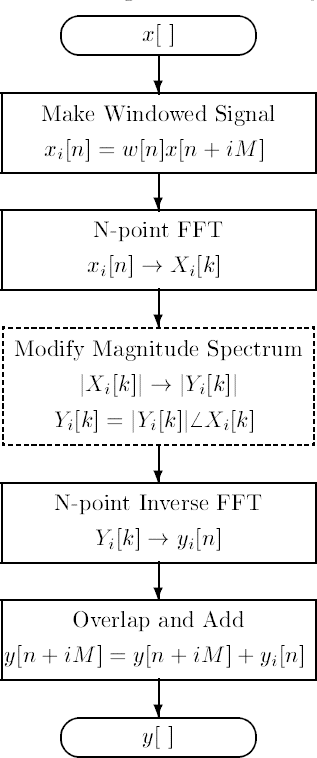
\includegraphics[scale=0.5]{resources/processing.PNG}
\par\end{centering}

\noindent \centering{}\caption{\label{fig:Block-diagrams-of}Block diagrams of how the samples are
processed. \citep{compernolle} }
\end{wrapfigure}%


\noindent Filtering of the noisy input signal is done primarily in
the frequency domain. This process is illustrated in \figref{Block-diagrams-of}.
The Fast Fourier Transform (DFT) algorithm is employed to perform
a Discrete Fourier Transform (DFT) on the input signal. Then assuming
that the noise is additive, the noise spectrum is estimated and subtracted
from the noisy signal. Finally, an inverse DFT (IDFT) is performed
on the input before sending it to the output.

Due to the real-time requirements of the system, it is not plausible
to take a DFT of the entire noisy input. Thus, frames are passed through
DFT and then processed accordingly. In order to prevent discontinuities
at frame boundaries (which manifest as clicking sounds heard in the
output), frames are processed in an overlapping manner, with appropriate
windowing done on the frames so that the overall gain at the frame
boundaries add up to unity. 


\subsection{\label{sub:Frame-Processing-Implementation}Frame Processing Implementation}

A frame size of 256 samples was chosen for frame processing, and an
oversampling ratio of four was chosen along the the square root of
the Hamming Window. This ensures that there are no sharp discontinuities
at frame edges and that the overall gain of the overlapped windows
sum to unity. This means that a full frame is taken for frequency
domain processing every $\nicefrac{1}{4}$ of a frame, known as a
frame segment. Each segment is thus 64 samples long. The processing
is illustrated in \figref{overlap-frame}.

\begin{figure}[H]
\noindent \begin{centering}
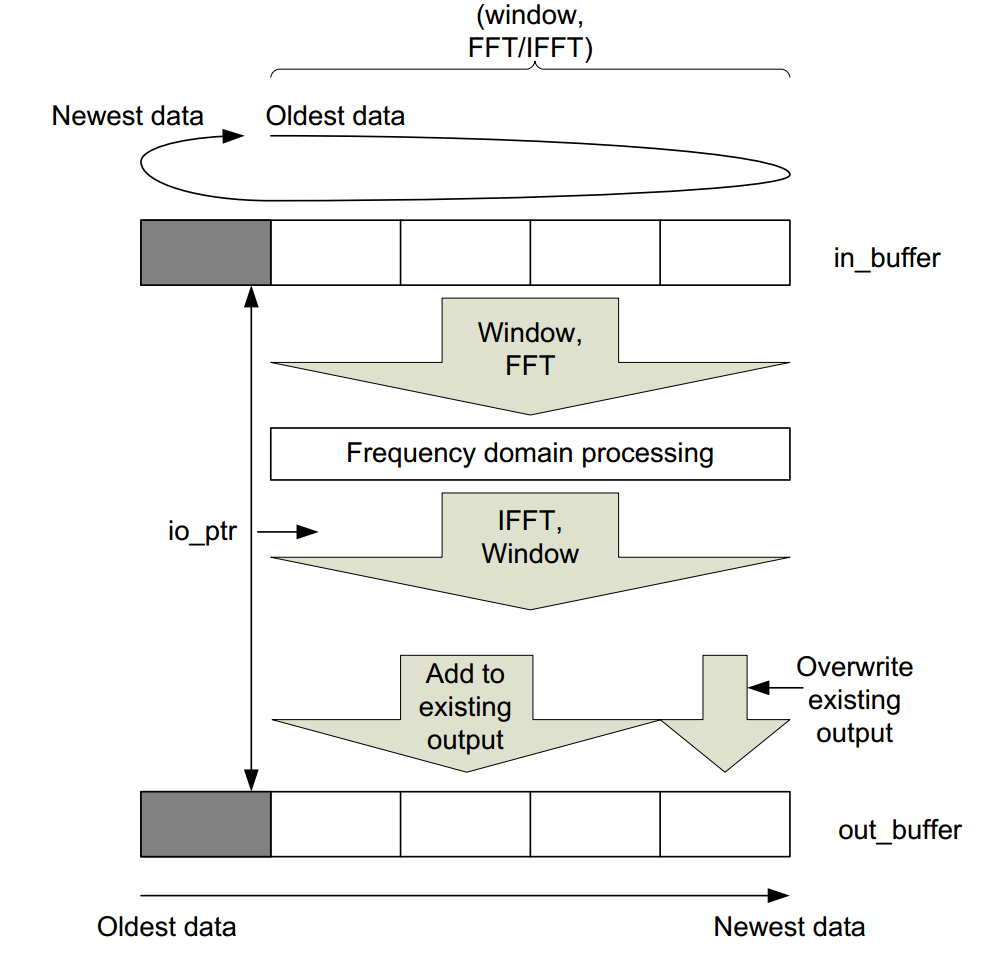
\includegraphics[scale=0.35]{resources/frame-overlap.PNG}
\par\end{centering}

\caption{\label{fig:overlap-frame}Implementation of the overlapped frame processing.
\citep{mitcherson}}


\end{figure}


The input and output buffer are implemented as circular buffers with
five segments each. At any time, four of those input segments will
be fully filled (and can be used for frame processing) with one being
used to store the inputs coming into the system. At the same time,
one of the output segments will have been fully added with its overlapped
frame (and therefore ready for output), while the other four frames
are being added with the current processed frame. The inputs are read
from the input port via an interrupt, and the relevant output is then
sent to the output port. This results in a 1.25 frame latency from
the input port to the output port. 


\subsection{\label{sub:Noise-Spectrum-Estimation}Noise Spectrum Estimation}

The heuristics used in the estimation of noise assumes that within
a 10 second window, the speaker would have at least paused for a fraction
of the time. During this time, the spectrum of the input would simply
correspond to that of the noise spectrum. Thus, the minimum of the
spectrum content over a ten-second sliding window can be used to estimate
the noise spectrum. Due to the fact that the phase of the noise spectrum
cannot be known, and the fact that slight phase distortion is not
audible to the human ears, only the absolute of the spectrum is analysed
and processed.

In practice, however, it is not feasible to store and minimise over
ten seconds worth of spectral content. Instead, the noise buffer is
split into four, each holding a minimum over a 2.5 second period.
These four separate noise minimum buffers are implemented as a single
circular buffer, with the appropriate program logic to separate the
segments. For the current window $M_{i}(\omega)$ (where $i\in[1,4]$
) and an input spectrum of $X(\omega)$, $M_{i}(\omega)=\min\left[|X(\omega)|,M_{i}(\omega)\right].$

When the noise spectrum is to be estimated for use in spectral subtraction,
the minimum over the four 2.5 seconds segments are used. Noting that
the nature of the naive noise estimation always underestimates the
noise content, therefore an over-subtraction factor $\alpha$ is used
for compensation. Thus, the minimum estimated noise spectrum $N(\omega)$
is given by
\begin{equation}
N(\omega)=\alpha\min_{i\in[1,4]}\left[M_{i}(\omega)\right]\label{eq:oversubtraction}
\end{equation}
where $\alpha$ was set to a value of 20 for the naive implementation,
producing a very aggressive filter. Although this is higher than the
suggested values by \citet{berouti}, it works decently in practice.
However, this results in high amplitude musical noise and some voice
distortion. Lowering $\alpha$ would let more noise through the filter,
but at the same time reduce the amount of musical noise (see section
\ref{sub:Musical-Noise}) present.


\subsection{\label{sub:Noise-Spectrum-Subtraction}Noise Spectrum Subtraction}

\begin{wrapfigure}[19]{O}{0.4\columnwidth}%
\noindent \begin{centering}
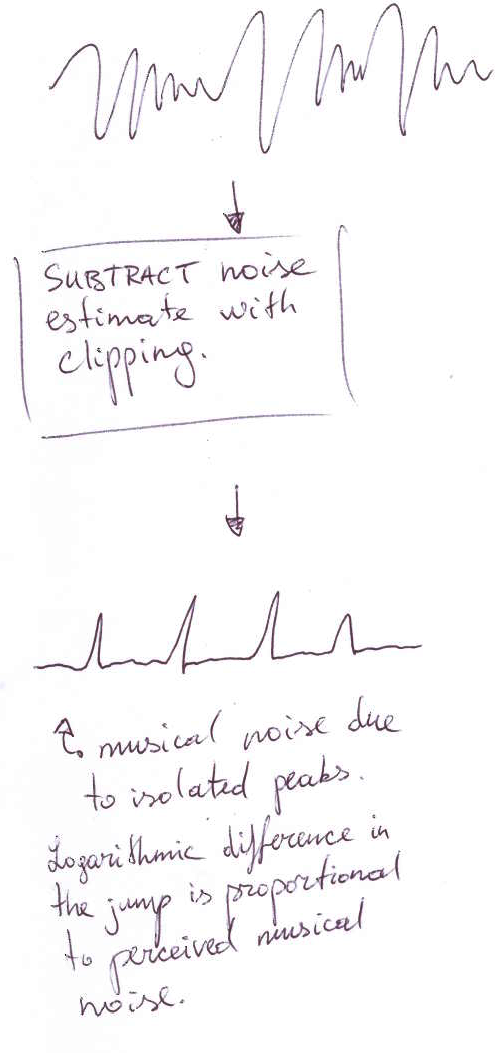
\includegraphics[scale=0.6]{resources/musical-noise}
\par\end{centering}

\caption{\label{fig:musical-noise-illus}Illustration of the generation of
musical noise by noise clipping.}
\end{wrapfigure}%


Let the output be $Y(\omega)$, and the input and noise be $X(\omega)$
and $N(\omega)$ respectively. To preserve the phase of $X(\omega)$
(and achieve a zero-phase filtering), only the magnitude should be
altered, as mentioned before. Thus, the output is given by
\begin{alignat}{1}
|Y(\omega)| & =|X(\omega)|-|N(\omega)|=|X(\omega)|\left(1-\frac{|N(\omega)}{|X(\omega)|}\right)\label{eq:1}\\
Y(\omega) & =X(\omega)G(\omega)\\
G(\omega) & =\max\left(\lambda,1-\frac{|N(\omega)|}{|X(\omega)|}\right)\label{eq:g_w}
\end{alignat}
where $G(\omega)$ is a gain factor that is calculated from the estimated
noise spectrum derived from \eqref{1}. Because of the fact that the
expression $1-\frac{|N(\omega)|}{|X(\omega)|}$ can potentially go
negative (i.e. the noise is overestimated), $G(\omega)$ should be
lower bounded. The input is not simply attenuated to zero (but to
the noise floor $\lambda$) to reduce the amount of perceivable ``musical
noise''. 


\subsubsection{\label{sub:Musical-Noise}Musical Noise}

When subtracting an estimate of the noise with clipping, imperfect
noise estimation produces isolated peaks in the spectrum of the filtered
signal, which is perceived as low-tone musical notes. This is illustrated
in \figref{musical-noise-illus}. As human sound perception is logarithmic
\citep{compernolle}, the difference between the zeroed floor and
a sharp peak is very pronounced. Instead, by clipping to a small positive
value $\lambda$, the differential step between the post-filter noise
floor ($\lambda)$ and the spectral peaks that are a result of imperfect
noise estimation can be reduced. In this basic implementation, the
spectral noise floor constant $\lambda$ was chosen to be 0.05 by
empirical methods, choosing from the ranges suggested by \citet{berouti}.
Generally, a higher $\lambda$ would result in a higher white noise
level, but lower perceived musical noise. Lower $\lambda$ results
in a lower white noise output but a more pronounced musical noise
effect.


\subsection{Evaluation}

\noindent 
\begin{figure}[H]
\noindent \begin{centering}
\subfloat[\label{fig:spec-clean}Spectrogram of the clean file]{\noindent \begin{centering}
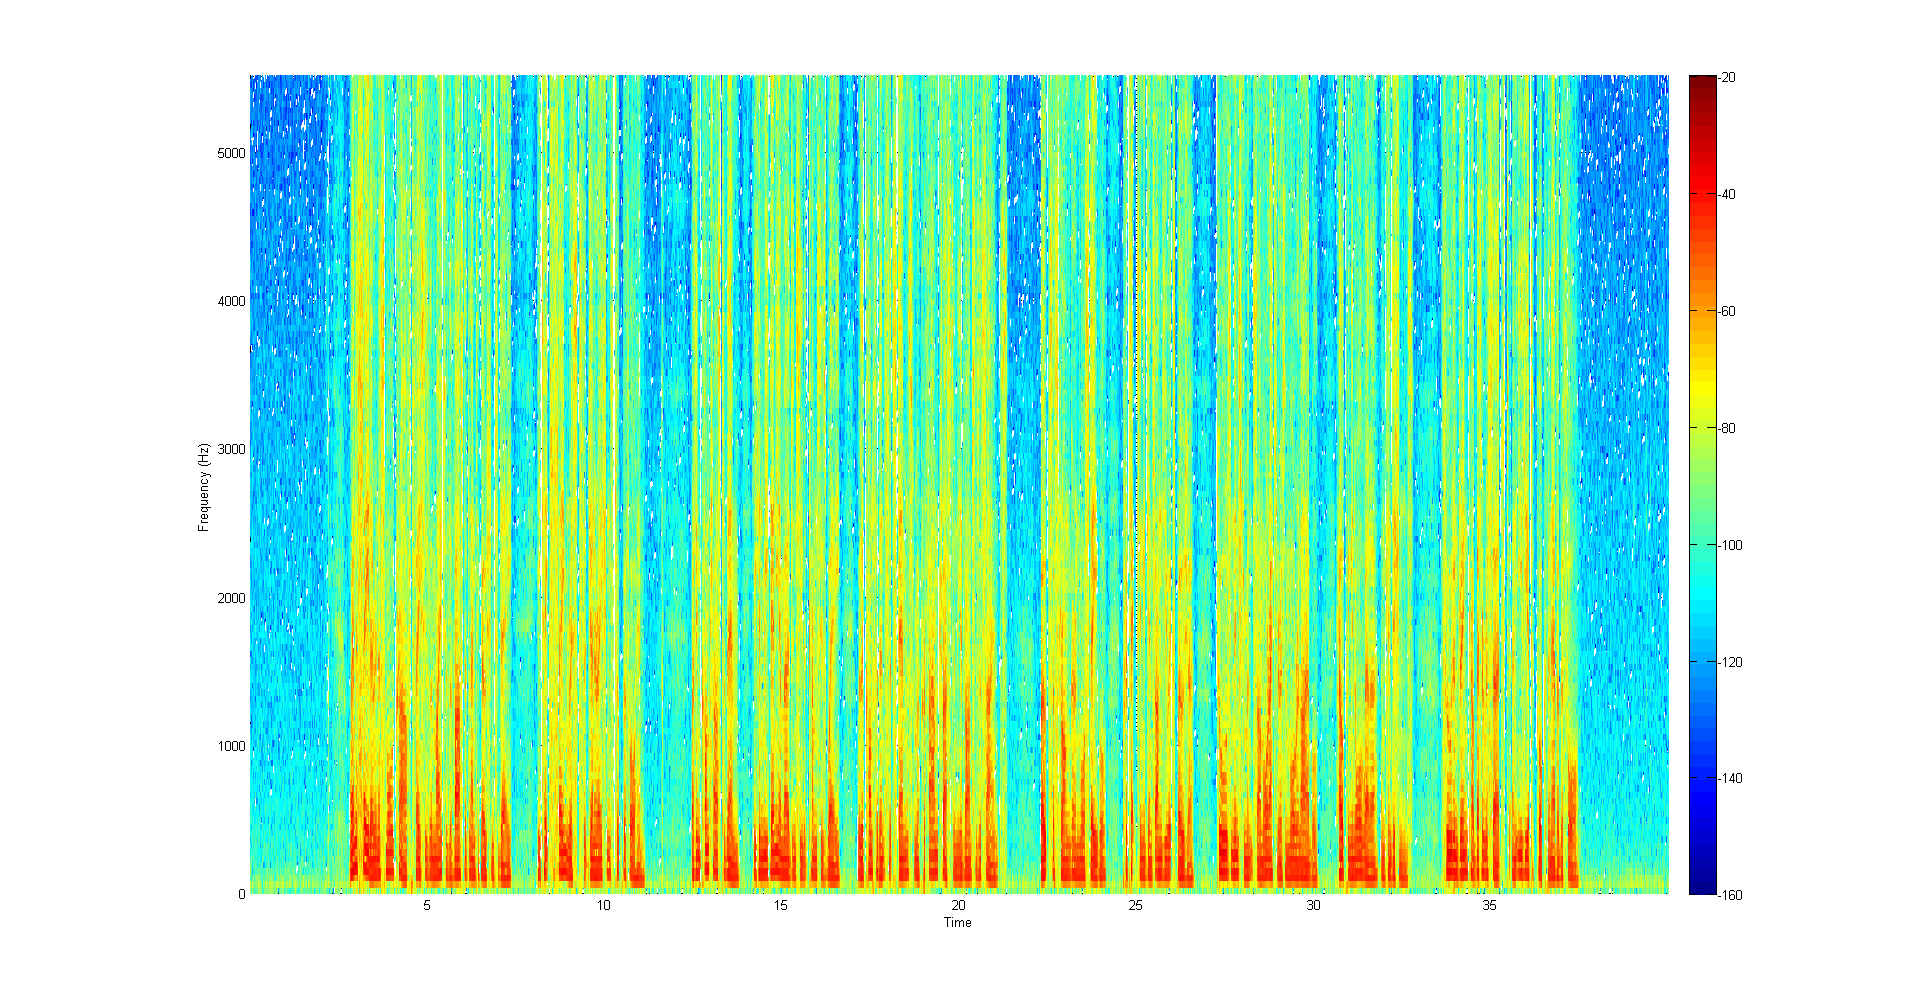
\includegraphics[scale=0.2]{resources/spec-clean}
\par\end{centering}

\noindent \centering{}}\hfill{}\subfloat[\label{fig:spec-factory2}Spectrogram of ``factory2'' file]{\noindent \begin{centering}
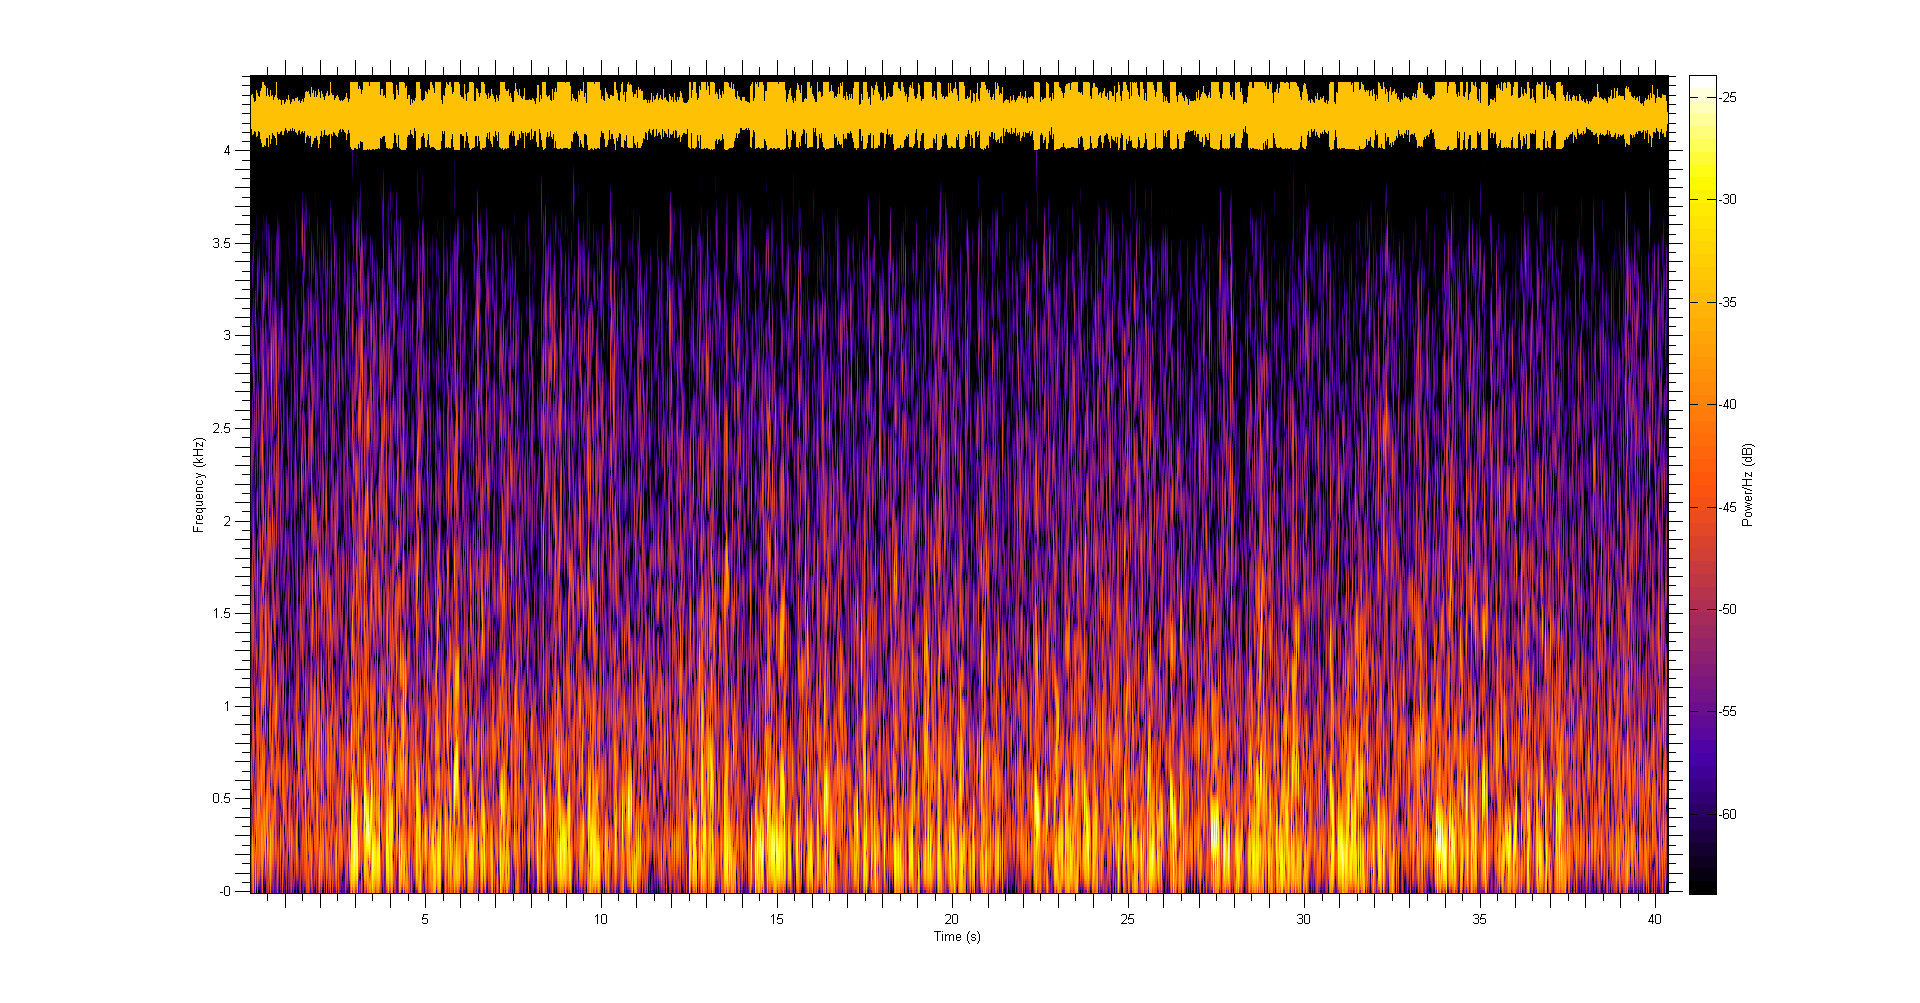
\includegraphics[scale=0.2]{resources/spec-factory2}
\par\end{centering}

\noindent \centering{}}
\par\end{centering}

\noindent \centering{}\caption{Spectrograms of provided files, generated in Matlab}
\end{figure}
 

\noindent As human perception of volume, noise and in general audio
signal clarity is very subjective and lacks a complete mathematical
model, spectrograms are used to introduce some form of objectivity
when evaluating the performance of the filter. The ``factory2''
corrupted sample is used for evaluation of the filter. Figure \ref{fig:spec-clean}
shows the spectrogram of the provided clean sound file, and \figref{spec-factory2}
shows the spectrogram of the ``factory2'' corrupted signal. 

\noindent 
\begin{figure}[H]
\noindent \begin{centering}
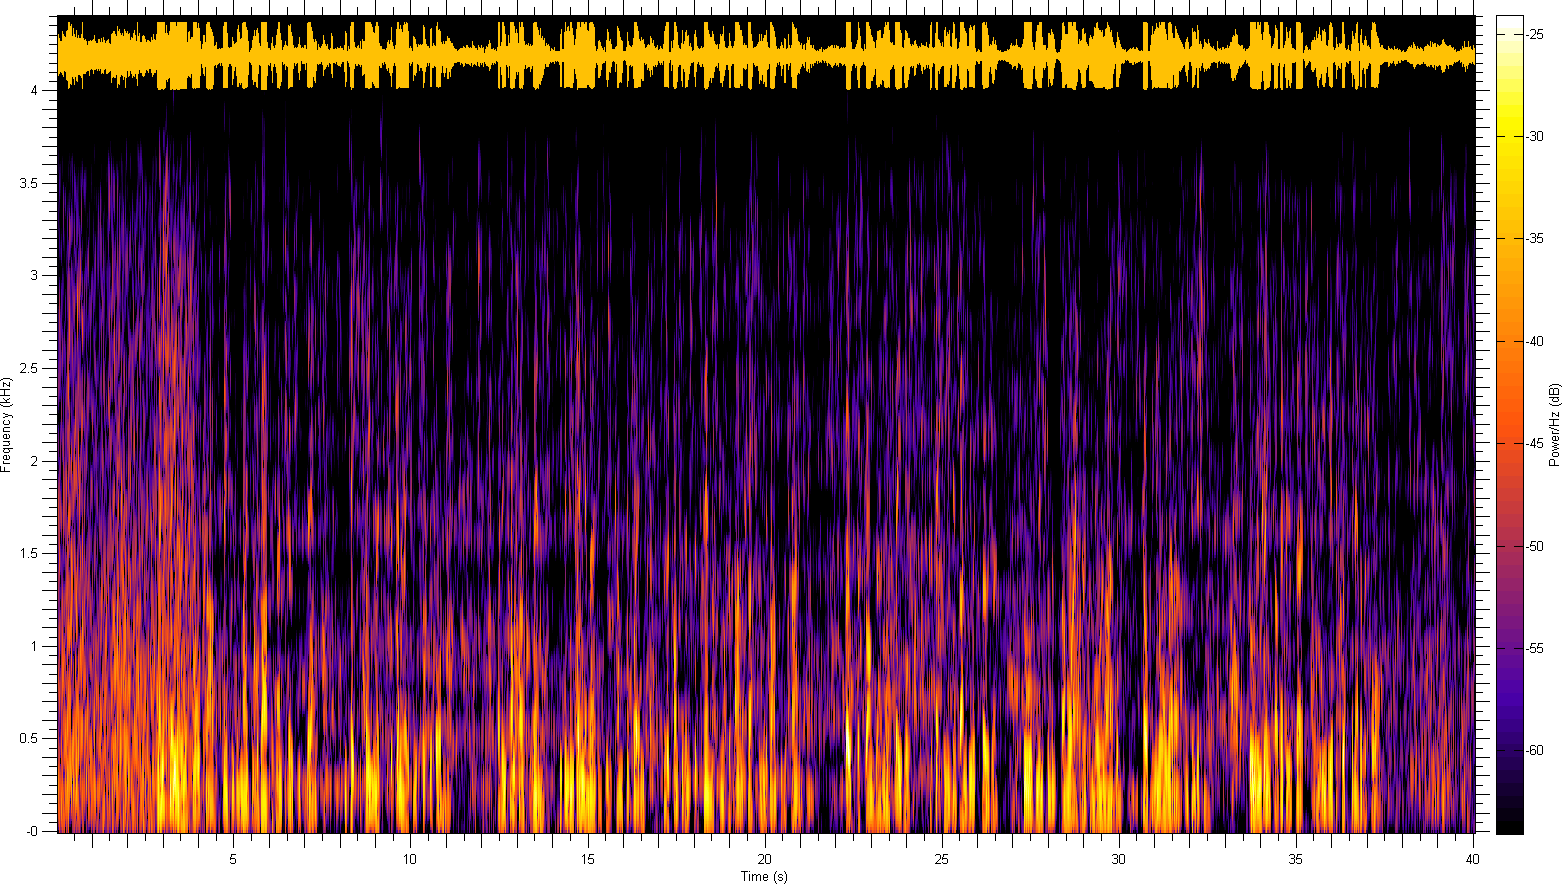
\includegraphics[scale=0.46]{resources/spec-no-enhancement}
\par\end{centering}

\caption{\label{fig:spec-no-enhancement}Spectrogram of the basic filtering
of ``factory2'' at 8000 Hz sampling frequency.}
\end{figure}


After applying the basic filter, the results can be seen in \figref{spec-no-enhancement}.
From listening tests, the basic implementation has managed to attenuate
the background noise slightly, with darker areas seen in \figref{spec-no-enhancement}
in between speech. The filter is slow in responding to background
noise changes, especially when the noise level transits from a low
level to a high level. This is due to the ten-second window used for
noise estimation. As the filter is always conservative about the noise
level being low (by always taking the minimum), the lower estimate
before the transition is always dominating until the relevant minimum
noise buffer is discarded. Due to the high over-subtraction factor
$\alpha$ introduced in \eqref{oversubtraction} to correct the underestimation
of noise, some of the speech is also removed and results in the voice
being slurry. There is also a very pronounced level of musical noise.

The unnatural sounding musical noise is a result of the magnitude
of the frequency exhibiting strong fluctuations in the noisy area
\citep{cappe}. Referring to \figref{spec-clean}, it can be seen
that the speech is paused between 11-12.5 s and the spectrogram is
completely empty during that period. In the filtered version in \figref{spec-no-enhancement},
it can be seen that there is noise during this period of time, and
the magnitude of the frequency bins fluctuates very rapidly, exhibiting
the musical noise effect mentioned above (see section \ref{sub:Musical-Noise}).


\section{\label{sec:sec-enhancement}Enhancements}

Various enhancements are implemented, and evaluated for their effectiveness
in removing the noise from the signal. Some of these enhancements
improve the noise removal, while some exacerbate the noise. Each are
thus evaluated in turn for their effectiveness, and a final combination
of these enhancements is described in \secref{Final-Implementation}. 


\subsection{\label{sub:complex-conjugate}Structural Optimisation}

The frequency spectrum processing can be sped up by slightly less
than a factor of two simply by only processing the first half, plus
one, of the frequency bins in the DFT. This is because the inputs
to the DFT are real, and thus the DFT of the inputs will be complex
conjugates around the middle. For our frame size of 256, where $X_{k}$
denotes the $k$\textsuperscript{th} frequency bin, $X_{256-i}=X_{-i}=X_{i}^{*}$
for $i\in[1,127]$, and $X_{0}$ and $X_{128}$ are simply real-valued.
This also allows some of the buffers used in the enhancements described
below to be almost halved in size.

This helps to prevent ``clicking'' in the output, resulting from
frame computation taking longer than one frame length. 


\subsection{\label{sub:Low-Pass-Filter-Input}Low-Pass Filter Input for Noise
Estimation}

\noindent 
\begin{figure}
\noindent \begin{centering}
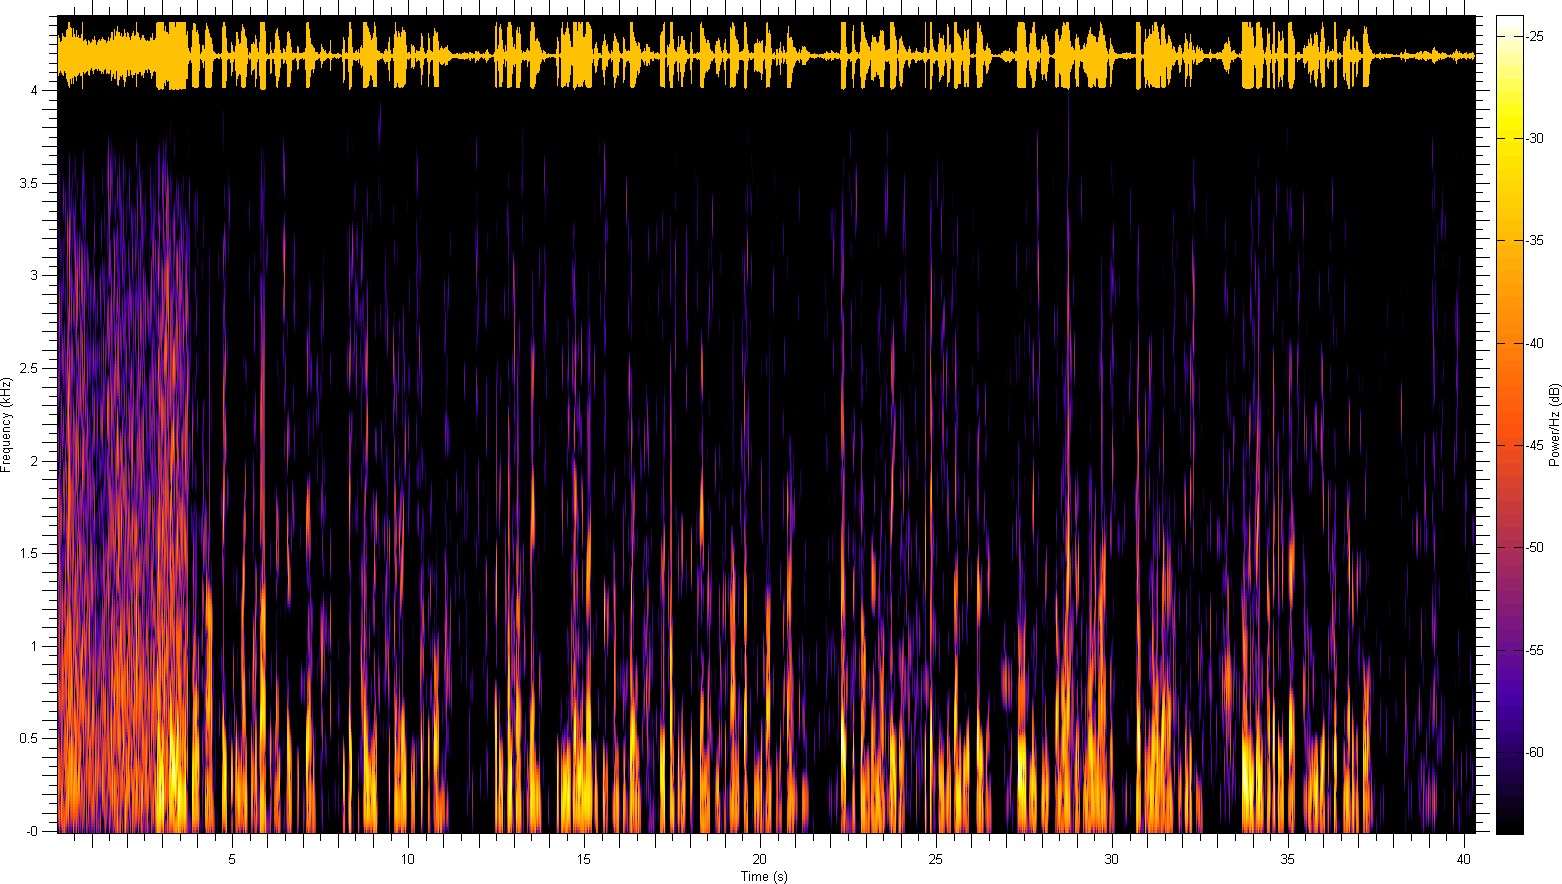
\includegraphics[scale=0.46]{resources/spec-enhancement-2}
\par\end{centering}

\caption{\label{fig:spec-enhancement-2}Spectrogram of the filtering with the
low-pass filter input for spectral content across time}
\end{figure}
A problem with the basic approach is that each frame's DFT is considered
alone when updating the estimate of the minimum noise. Therefore,
even a single frame with an instantaneous magnitude drop for an DFT
bin will potentially stay as the overly conservative noise estimate
for the duration of the noise buffer. Since the frame length for 256
samples at 8000 Hz sampling frequency is 32 ms, one particularly underestimated
noise value will stay within the minimum noise buffer for a period
that can last seconds. This is the reason for a high over-subtraction
coefficient for the basic filter above, to compensate for the filter's
conservatism of the noise level. Furthermore, for the same reasons
of the filter being overly optimistic, any noise with small spectral
pauses (that need not be aligned to one frame) will defeat the basic
implementation.


\subsubsection{Magnitude domain}

One way of improving on the naive spectral subtracter is to low-pass
filter (LPF) the DFT magnitude bins across time according to:
\begin{eqnarray}
P_{t}(\omega) & = & (1-k)\times|X(\omega)|+k\times P_{t-1}(\omega)\label{eq:lpf-input}\\
k & = & e^{(-\nicefrac{T}{\tau})}
\end{eqnarray}
where $P_{t}$ is the input estimate to be presented to the minimum
noise buffer as per \eqref{oversubtraction}, $T$ is the frame rate
(the time between frame calculation), and $\tau$ is the time constant
parameter for this filter. 

$P_{t}(\omega)$ is the low pass filtered DFT bin that corresponds
to the persistent average level of the magnitude at that frequency
bin, with the smoothness of the filtering controlled by the time constant
$\tau$. By taking the minimum of the low pass filtered signal as
the noise minimum (\eqref{oversubtraction}), the filter will not
suffer from the degenerating upon encountering sudden magnitude jumps
in the noise signal's spectral content. Result is such that the noise
buffer's noise estimate now more closely matches the persistent noise
level. This is illustrated in \figref{lpf-illus}.

\begin{wrapfigure}{O}{0.5\columnwidth}%
\noindent \begin{centering}
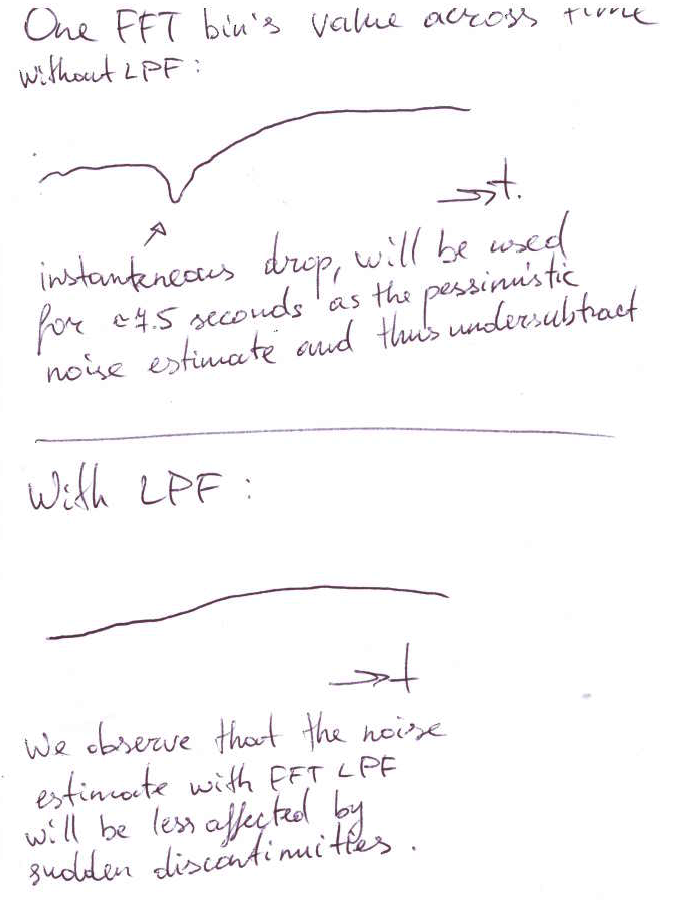
\includegraphics[scale=0.6]{resources/lpf}
\par\end{centering}

\caption{\label{fig:lpf-illus}Illustration of the low pass filtering of the
DFT bins.}
\end{wrapfigure}%


The over-subtraction coefficient, $\alpha$, can thus be reduced from
20 to 3.2. This also reduces the musical noise perceived by lowering
the level of fluctuation in the magnitude at each frequency bin between
clipped and unclipped samples. This is due to the subtracted spectrum
being more closely matched to the actual noise level.

In the basic filter, when the input $|X(\omega)|$ falls sharply,
this would cause a sharp fall in $|N(\omega)|$ and cause a discontinuity
in the output. Low pass filtering removes this discontinuity by introducing
a smoother transition. This also has the effect of lowering the responsiveness
of the filter, but is worth the trade-off due to much better noise
estimation.

The low pass filter can also be seen as a system where the inputs
are integrated over a period of time and then averaged. Therefore,
by having a longer period to average over, the pauses between speech
can be used to get a much more accurate average noise estimate. Figure
\ref{fig:spec-enhancement-2} shows the output of the filter being
more successful in filtering out the noise when compared to \figref{spec-no-enhancement}.
This is because the filter is now less susceptible to problems caused
by a momentary drop in the input. The amount of musical noise is also
significantly reduced as well (for example in the pause in speech
from 11-12.5s).

The time constant factor $\tau$ can be adjusted in this filter, and
50 ms was chosen for the implementation. This value was obtained empirically
through blind listening tests with the set of samples given in the
range of 20 to 80 ms. This range maximises the integration period
of noise by being matched with the inter-word pause timings. Having
a higher time constant results in a longer integration period, which
when bigger than the pauses between words will start integrating voice
spectrum as part of the noise estimate. A higher $\tau$ also means
a slightly slower response to noise level change, although the 7.5
seconds period of the full noise buffer rotation latency has a bigger
effect on the response speed (see section \ref{sub:Noise-Spectrum-Estimation}).
A smaller $\tau$ on the other hand will be similar to the basic implementation
through averaging over a shorter period.


\subsubsection{Power domain}

Alternatively, the LPF of the frequency bins can be done in power
domain:
\begin{equation}
P_{t}(\omega)=\sqrt{(1-k)\times|X(\omega)|^{2}+k\times\left[P_{t-1}(\omega)\right]^{2}}\label{eq:power-lpf}
\end{equation}
Power domain filtering provides slightly more accurate filtering,
because human hearing tracks the power of the signal closer than its
magnitude. Hence, the perceivable noise could potentially be reduced.

An approach where the entire noise estimation and noise subtraction
is performed in the power domain was explored, converting to magnitude
domain only before output. Thus, \eqref{power-lpf} becomes
\begin{equation}
P_{t}(\omega)=(1-k)\times|X(\omega)|^{2}+k\times P_{t-1}(\omega)
\end{equation}
and noise subtraction originally in the form of \eqref{eq2} can be
performed by
\begin{equation}
|Y(\omega)|=\sqrt{|X(\omega)|^{2}-|N_{p}(\omega)|}
\end{equation}
where $|N_{p}(\omega)|$ is the minimum noise estimate in the power
domain estimated in the same way as in \eqref{oversubtraction} .

Testing showed no perceivable difference regardless of whether the
filtering was done in the magnitude or power domain (including both
variants), agreeing with \citet{compernolle}.


\subsection{\label{sub:enhancement-3}Low-Pass Filter Noise Estimate}

Another potential for discontinuities in the output is when the minimum
noise buffers are rotated. These steps can be perceivable if the noise
level changes significantly. They can be smoothed out by low pass
filtering over the noise estimates. This ensures a smoother transition
between noise buffer rotations. The filtering is done by 
\begin{eqnarray}
|N_{lpf}(w)| & = & (1-k_{n})\times|N(w)|+k_{n}\times|N_{lpf}(w)|\\
k_{n} & = & e^{(-\nicefrac{T}{\tau_{n}})}
\end{eqnarray}
where $\tau_{n}$ is the time constant for this low pass filter. The
time constant determines how smooth,and less responsive the transitions
will be, with higher time constant giving a smoother transition. 

Experimental testing showed that $\tau_{n}=100\unit{ms}$ gave the
best performance for the samples given.


\subsection{\label{sub:alt-gw}Alternate Calculation for $G(\omega)$}

\begin{comment}
adaptive noise floor level based on SNR

1 - n/p 
\end{comment}


\begin{figure}
\noindent \begin{centering}
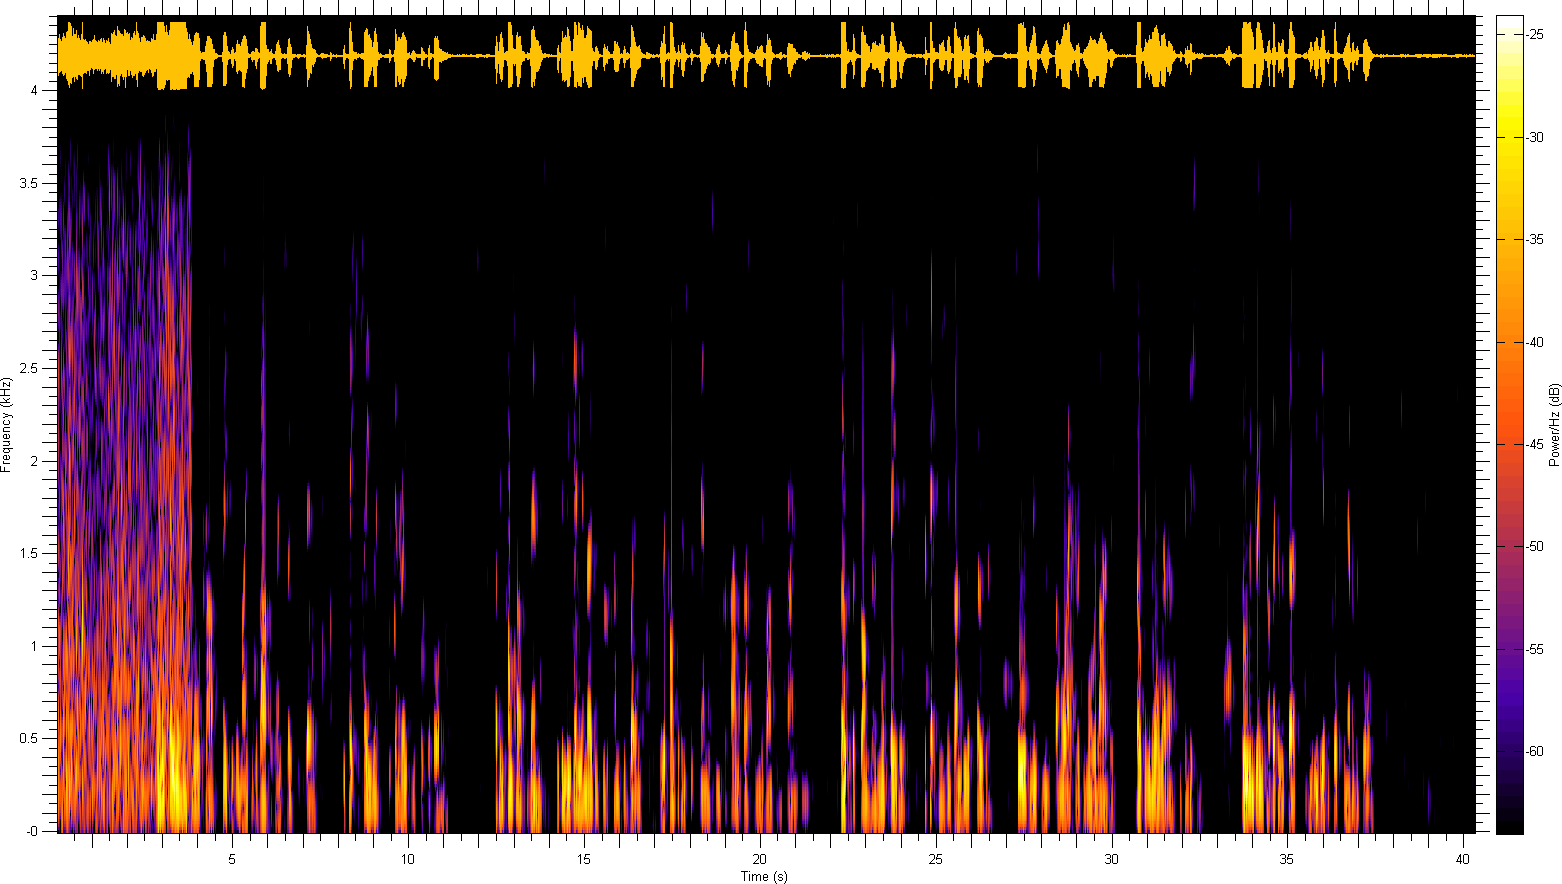
\includegraphics[scale=0.46]{resources/spec-enhancement-2-4}
\par\end{centering}

\caption{\label{fig:spec-enhancement6}Spectrogram using an alternate calculation
for $G(\omega)$, combined with input LPF for noise estimation}
\end{figure}


The nature of the noise estimation algorithm is such that a lower
noise estimate (even momentarily) will cause an underestimate of the
noise spectrum. While this effect is moderated partly by the LPF in
section \ref{sub:Low-Pass-Filter-Input}, it still does not handle
situations where the noise level increases. Consider that the factor
$G(\omega)$ derived in \eqref{g_w} can be calculated using another
form to perform noise subtraction form the input $X(\omega)$:
\begin{alignat}{1}
\left|Y(\omega)\right| & =\left|X(\omega)\right|-|X(\omega)|\frac{\left|N(\omega)\right|}{\left|P(\omega)\right|}=\left|X(\omega)\right|\left(1-\frac{\left|N(\omega)\right|}{\left|P(\omega)\right|}\right)\label{eq:eq2}\\
\therefore G(\omega) & =\max\left[\lambda,1-\frac{\left|N(\omega)\right|}{\left|P(\omega)\right|}\right]
\end{alignat}
where $|N(\omega)|$ is the current minimum noise estimate over ten
seconds from \eqref{oversubtraction}, and $|P(\omega)|$ is the low-pass
filtered noise estimate for the current frame being processed from
\eqref{lpf-input}. \eqref{eq2} gives rise to different effects depending
on the values of $|N(\omega)|$ and $|P(\omega)|$.


\subsubsection{Noise Level Matches Minimum Estimate}

Consider a situation when the value of $|N(\omega)|$ is equal, or
slightly more than$|P(\omega)|$. This will signify that the current
minim noise estimate over ten seconds roughly matches the low-pass
filtered noise estimate for the current frame being processed. Thus,
there is a high confidence that the input $X(\omega)$ consists entirely
of only noise. Hence, the fraction $\frac{\left|N(\omega)\right|}{\left|P(\omega)\right|}\approx1$
and the entirety of $X(\omega)$ will be subtracted.


\subsubsection{Noise Level Increase}

Consider that $|N(\omega)|$ remains constant at a previously encountered
minima and that the noise level has increased via an increase in $|X(\omega)|$.
Then, because of the LPF in section \ref{sub:Low-Pass-Filter-Input},
$|P(\omega)|$ does not rise sharply, but slowly. Thus, $|P(\omega)|$
is slightly more than $|N(\omega)|$ and $\frac{\left|N(\omega)\right|}{\left|P(\omega)\right|}$
will have a value that is close to one. In the original form of noise
subtraction in \eqref{1}, $|X(\omega)|$ will continued to be subtracted
by a very low $|N(\omega)|$ while the noise level has risen. This
causes the increased noise to not be filtered, and can cause musical
noise. In \eqref{eq2}, this will result in a faster reduction in
noise as $|X(\omega)|$ will be subtracted by a larger value. A numerical
example of this happening is illustrated in \tabref{g-w-numerical}.

\begin{wraptable}[12]{O}{0.5\columnwidth}%
\noindent \begin{centering}
\begin{tabular}{|c|c|}
\hline 
$|N(\omega)|=0.1,|X(\omega)|=0.9$ & $|X(\omega)|-|N(\omega)|=0.8$\tabularnewline
\hline 
$|P(\omega)|$ & $|X(\omega)|-|X(\omega)|\frac{||N(\omega)|}{|P(\omega)|}$\tabularnewline
\hline 
\hline 
0.2 & 0.45\tabularnewline
\hline 
0.3 & 0.6\tabularnewline
\hline 
0.4 & 0.675\tabularnewline
\hline 
0.5 & 0.72\tabularnewline
\hline 
0.6 & 0.75\tabularnewline
\hline 
0.7 & 0.771429\tabularnewline
\hline 
0.8 & 0.7875\tabularnewline
\hline 
0.9 & 0.8\tabularnewline
\hline 
\end{tabular}
\par\end{centering}

\caption{\label{tab:g-w-numerical}Numerical example depicting the noise subtraction
during an increase in the noise level.}
\end{wraptable}%


However, as time goes by and $P(\omega)$ increases, $\frac{\left|N(\omega)\right|}{\left|P(\omega)\right|}\rightarrow|N(\omega)|$
as $|P(\omega)|\rightarrow1$. This means that, given sufficient time,
\eqref{eq2} will perform as badly, or even worse as \eqref{1} in
the event of a noise increase. Thus, the time constant $\tau$ in
\eqref{lpf-input} can be increased to slow down this process so that
eventually when the noise buffer described in section \ref{sub:Noise-Spectrum-Estimation}
rotates, the old value will be discarded. Alternatively, the time
interval in which the minimum noise is estimated across can be reduced.


\subsubsection{Evaluation}

The caveat with this enhancement is that $|P(\omega)|$ is unable
to distinguish speech from noise, and thus will cause some of the
speech to be removed as well.

The output with this enhancement implemented can be seen in \figref{spec-enhancement6}.
When compared with the results from \figref{spec-enhancement-2},
it can be seen that more noise (and musical noise) has been removed.
It can be noted that the noise in the period 11-12.5 s when the speaker
has paused his speech is almost fully removed. However, it is also
observed that some of the speech has also been removed, resulting
in a slightly slurry voice. 


\subsection{\label{sub:enhancement-7}Frame lengths}

In general, frame lengths should be of powers of two so that the Fast
Fourier Transform (FF) used for DFT can be the most efficient. The
frame length can be increased to give a better frequency resolution
when doing the DFT of the samples. This would give a more granular
approach in processing the frequency bins. However, this comes at
the expense of temporal resolution, although it is not as important
in this system. Due to the use of the frame processing structure described
in section \ref{sub:Frame-Processing-Implementation}, there is a
1.25 frame delay between the input and output, and increasing the
frame length will increase the time delay more. The increase in frame
length will also cause more processing to be done per frame, and if
the increased processing takes up more time than the frame time interval,
it would cause ``clicking'' to be heard in the final output. The
increase in frame length would also increase the heap memory used,
and the limited memory would be a limiting factor.

Through experimentation, it was found that increasing the frame length
did not yield much noticeable improvements. Reducing the frame length
caused a degradation in the filter quality, as the frequency resolution
would be reduced. It is noted that a frame length of 256 provides
sufficient granularity for a sampling rate of 8 kHz.

\begin{comment}
time resolution vs frequency resolution (and memory/computation)

I think that because the filter has already 3s lag or so, going from
32 to 64 ms frame length is not a significant time domain loss.

From experimentation, no significant difference between 256 and 512
observed though

http://electronics.stackexchange.com/questions/12407/what-is-the-relation-between-DFT-length-and-frequency-resolution
\end{comment}



\subsection{\label{sub:enhancement-6}Dynamic Over-subtraction}

The over-subtraction factor $\alpha$ described in \eqref{oversubtraction}
can be dynamically adjusted based on the signal to noise ratio (SNR)
given by $\frac{|X(\omega)|}{|N(\omega)|}$. When the SNR falls below
a certain threshold, the over-subtraction factor $\alpha$ can be
increased to cause more of the spectrum to be subtracted. It is known
that in the frequency range of 0-50 Hz, no human speech is present.
Thus, this frequency range is considered for increased over-subtraction.
Alternatively, instead of over-subtracting and allowing these frequency
bins to fall to the noise floor level, $\lambda$ (see \eqref{g_w}),
these frequency bins can simply be zeroed.

Through experimentation, with a low SNR threshold (approximately 2),
no discernible difference could be heard and the spectrogram output
did not reflect much improvement. When the SNR threshold was raised
(to about 5), a degradation in the speech could be heard. This is
because the noise level $|N(\omega)|$ is simply a minimum estimate
and does not discern between noise and speech. When the 0-50 Hz frequency
bins were simply zeroed, some of the low frequency musical noise was
eliminated (e.g. in input ``car''), and no degradation in speech
was perceived.

\begin{comment}
<enh6?>

the main spectral content of human speech can be assumed to be between
50 and 8000 Hz. 

Therefore one possible improvement is to over-subtract 0-50 Hz band
even further.

We also explored completely zeroing the 0-50 Hz band, results were
<ok? do a quick test>

When listening to filtering of ``car1.wav'' corrupted signal with
a pair of high quality headphones, the low frequency components could
actually be heard leaking into the signal. This additional over-subtraction
helped combat this effect.
\end{comment}



\subsection{\label{sub:enhancement-8}Residual Musical Noise Reduction}

\begin{figure}[H]
\noindent \begin{centering}
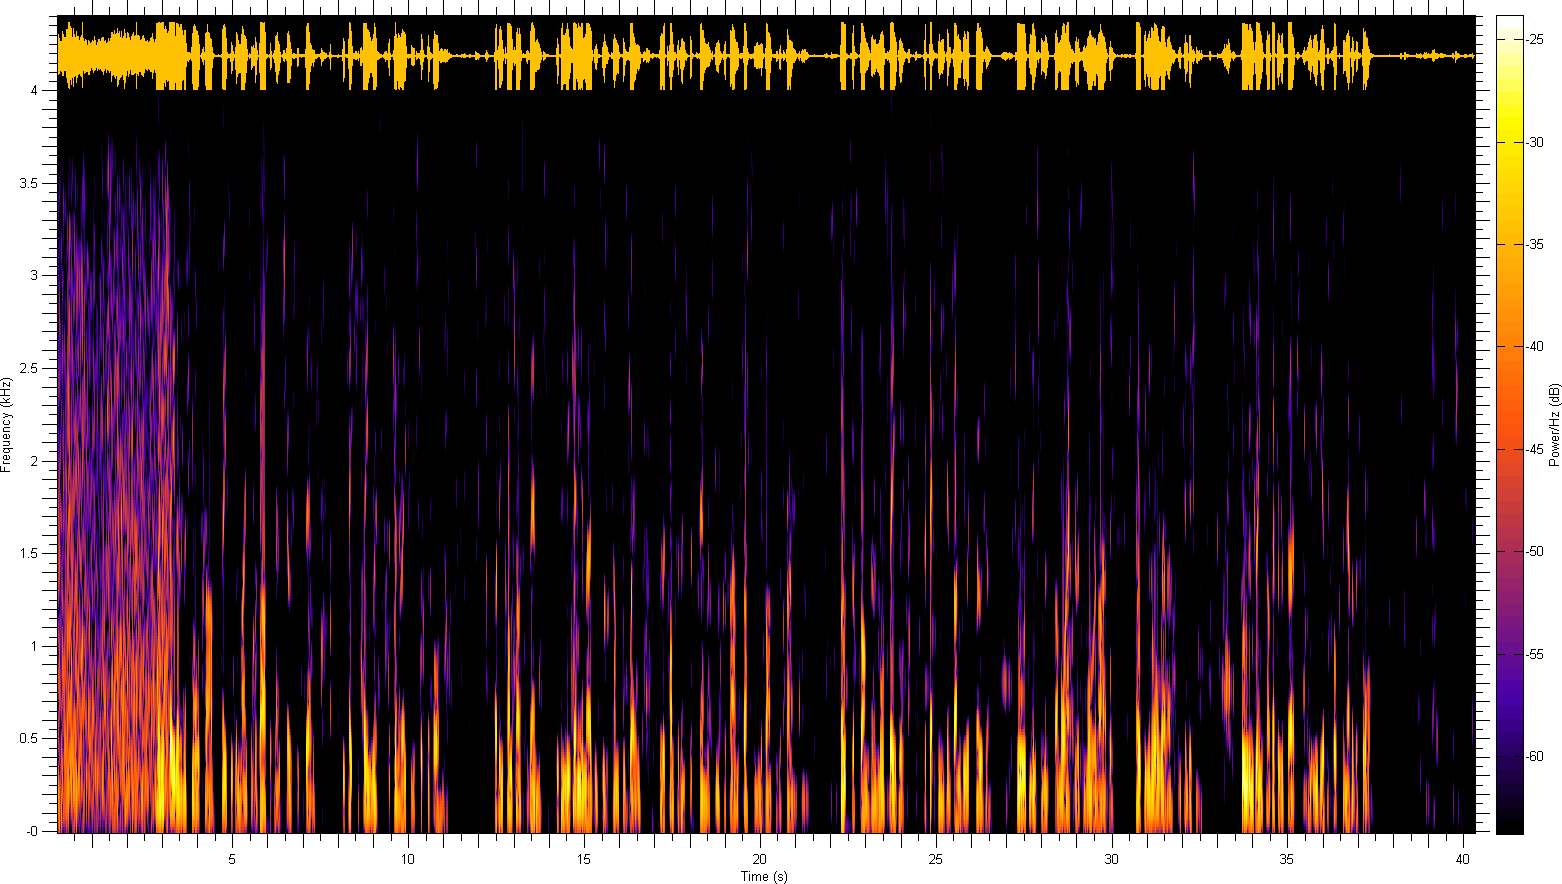
\includegraphics[scale=0.46]{resources/spec-enhancement-8}
\par\end{centering}

\noindent \begin{centering}
\caption{\label{fig:spec-enhancement-8}Spectrogram of the output with residual
musical noise reduction.}

\par\end{centering}

\end{figure}


The residual musical noise (see section \ref{sub:Musical-Noise})
can be suppressed further. For a specific frequency bin, the musical
noise is due to random fluctuation in its amplitude across different
frames, therefore, it can be replaced with its minimum value from
adjacent frames \citep{boll}. 

For a current frame $k$, if the ratio $\nicefrac{|N(\omega)|}{|X(\omega)|}$
is high, more noise is estimated than there is input. Then, take the
output $|Y(\omega)|=\min_{i\in\{k-1,k,k+1\}}\left[|Y_{i}(\omega)|\right]$.
The motivation for doing so is that if $\nicefrac{|N(\omega)|}{|X(\omega)|}$
is high and $|X(\omega)|$ is rapidly fluctuating, then there is a
high probability that it is simply noise, and can be minimised. If
$|X(\omega)|$ is constant, it is likely to be low energy speech.
Therefore, taking the minimum will retain the speech content. 

It should be noted that this would require the low-pass filtering
described in section \ref{sub:Low-Pass-Filter-Input} to be implemented.
Otherwise, every time $|X(\omega)|$ goes lower than $|N(\omega)|$,
$|N(\omega)|$ will simply be updated with this new value. The LPF
smooths out the sharp drops, thus allowing $\nicefrac{|N(\omega)|}{|X(\omega)|}$
to go above one.

Generally, the threshold for $\nicefrac{|N(\omega)|}{|X(\omega)|}$
should be high so that rapidly fluctuating noise can be filtered out.
However, if the threshold is too high, the minimisation might not
kick in often enough because $|N(\omega)|$ would simply ``catch
up'' with the lower value of $|X(\omega)|$. Increasing the time
constant $\tau$ in \eqref{lpf-input} would allow the threshold to
go higher. A lower threshold would cause less fluctuating noise to
be removed.

The spectrogram of the output for a threshold of 3 can be seen in
\figref{spec-enhancement-8}. Compared with the output from \figref{spec-enhancement-2},
it can be seen that more of the musical noise (c.f. 11-12.5s) has
been removed. 


\subsection{\label{sub:enhancement-9}Changing the Noise Estimation Period}

The noise estimation window described in section \ref{sub:Noise-Spectrum-Estimation}
can be reduced to allow the noise filter to react faster to changes
(especially increase) in noise level. This will also allow the alternate
$G(\omega)$ calculation described in section \ref{sub:alt-gw} to
perform better due to the faster rotation of the noise buffers. However,
if the speaker does not pause at all during the period, his voice
at its lowest level will be taken as noise and then erroneously subtracted
from the spectrum as a result of estimating noise over a shorter time
period. 

\begin{comment}
quicker tracking vs potentially filtering voice out if it stays audible
for long periods of time,

quicker tracking -> more relevant noise pattern -> better filtering
for changing noise

<elaborate on trade-off?>
\end{comment}
{} By analysing the spectrogram of the clean version of the sound file
(see \figref{spec-clean}), it can be seen that the speaker does pause
at least once every four seconds (however short). Therefore the total
length of all the noise buffers combined contributes to 4 seconds
in our implementation.


\section{\label{sec:Final-Implementation}Final Implementation}

\noindent \begin{wraptable}{O}{0.5\columnwidth}%
\noindent \begin{centering}
\begin{tabular}{|c|c|}
\hline 
Quantity & Value\tabularnewline
\hline 
\hline 
Over-subtraction factor, $\alpha$ & 3.2\tabularnewline
\hline 
Noise floor, $\lambda$ & 0.05\tabularnewline
\hline 
Input LPF time constant, $\tau$ & 0.05s\tabularnewline
\hline 
Noise Estimate LPF time constant, $\tau_{n}$ & 0.1s\tabularnewline
\hline 
\end{tabular}
\par\end{centering}

\caption{\label{tab:parameter}Parameters for the final implementation.}
\end{wraptable}%


In the final implementation of the filter, the enhancements described
in sections \ref{sub:complex-conjugate}, \ref{sub:Low-Pass-Filter-Input},
\ref{sub:enhancement-3}, \ref{sub:alt-gw}, \ref{sub:enhancement-6},
and \ref{sub:enhancement-9} were implemented. The structural optimisation
described in section \ref{sub:complex-conjugate} was implemented
to improve the computational performance of the filter. 

The input low pass filtering enhancement described in section \ref{sub:Low-Pass-Filter-Input}
gave the most significant improvement in terms of musical noise reduction.
The alternate $G(\omega)$ calculation described in section \ref{sub:alt-gw}
improves upon the LPF by addressing its shortcomings. This requires
that $\tau$ be set to a slightly higher value. The noise estimation
period (section\ref{sub:enhancement-9}) was also reduced to four
seconds to improve the performance of the alternate $|G(\omega)|$
calculation and increase the response rate of the filter. The frequency
bins for 0-50 Hz were also zeroed, as described in section \ref{sub:enhancement-6}
because no human speech spectral content in that band is insignificant. 

The enhancement described in section \ref{sub:enhancement-7} was
not implemented due to the adverse effects on the output. The enhancement
described in section \ref{sub:enhancement-8}, while achieving good
results, requires a longer $\tau$ to further improve the results
already gotten from the other enhancements, and this will cause the
noise estimate to be slower in reacting to changes. 

The spectrogram of the output with enhancements combined can be found
in \figref{spec-final}, and the parameters used can be found in \tabref{parameter}.
The filter has removed the musical noise present during periods when
speech is paused significantly (for example 11-12.5s) due to the filter
being able to better react to changing noise levels. It has also reduced
the amount of high frequency noise. 

\begin{figure}[H]
\noindent \begin{centering}
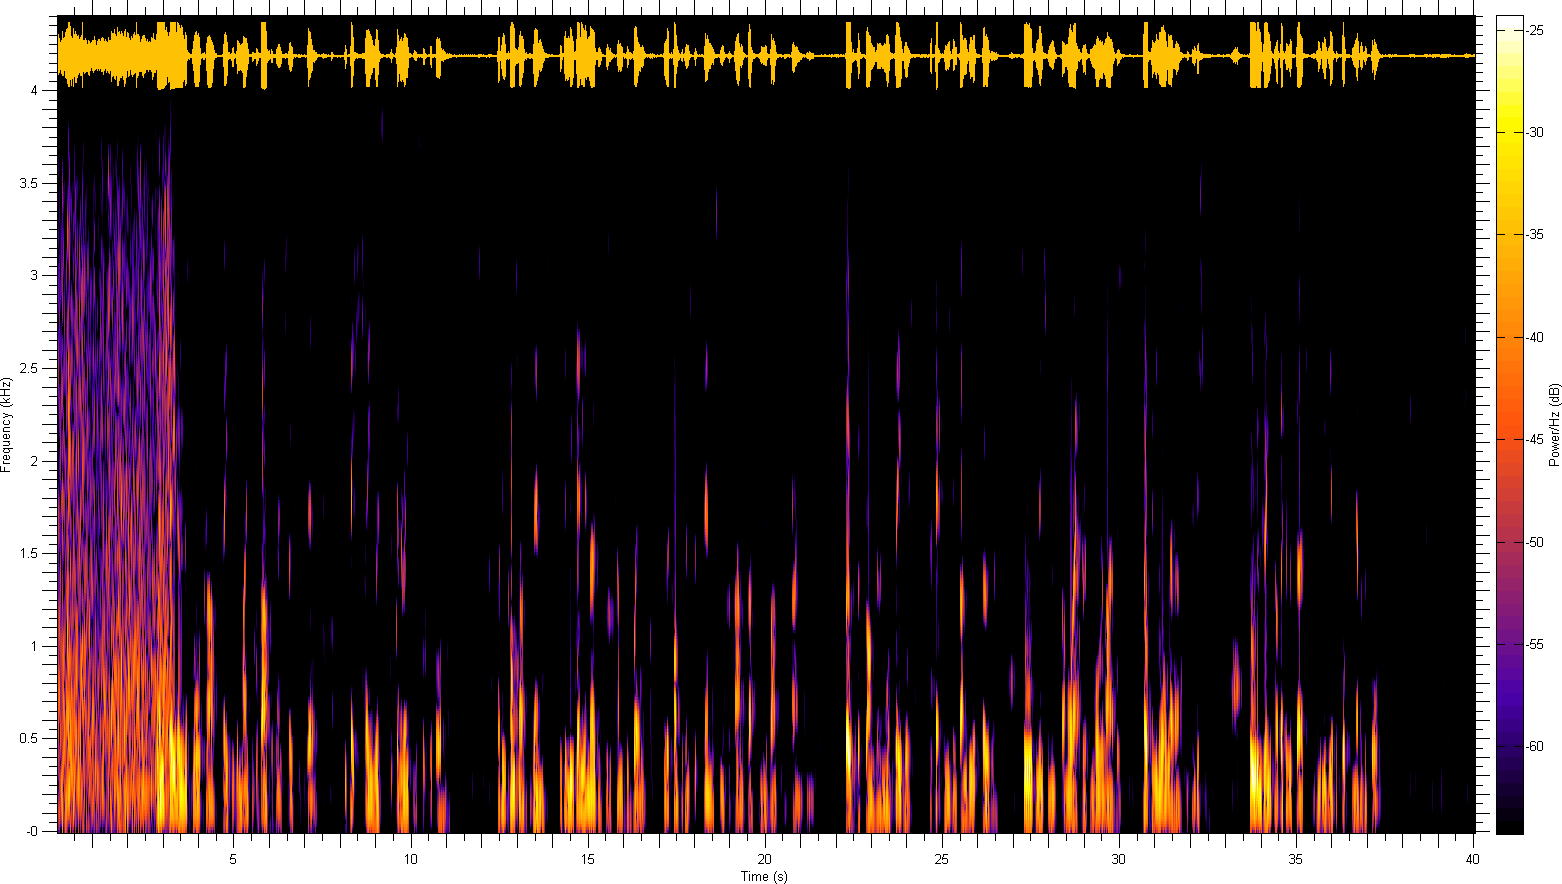
\includegraphics[scale=0.46]{resources/spec-enhancement-combined}
\par\end{centering}

\caption{\label{fig:spec-final}Spectrogram of the filtered signal for the
final implementation.}


\end{figure}



\section{\label{sec:further}Further ideas}

A very appropriate application of spectral subtraction is mobile telephony
due to its simplicity and low computational requirements. In such
an application, when the connection for a call is initially established,
the caller is not expected to immediately start speaking. As such,
the first brief period after establishing a connection can be treated
as being pure background noise. Noise can therefore be estimated before
speech begins. This could be implemented by simply filling up the
noise buffers with the initial samples and then continuing the estimation
as before. This will remove the initial ``warm up time'' that the
filter experience due to the way the noise buffers are set up in section\ref{sub:Noise-Spectrum-Estimation}.
Thus, the person on the other end of the line will receive a filtered
output right from the beginning. Additionally, the filter could start
tracking the noise even during the connection set-up delay period.

Another trait of mobile telephony is that usually a device will usually
only have one or very few associated users. Therefore adaptive filters
that are trained to perform better based on the principal traits of
the owner's speech can be implemented. This could be achieved in a
variety of ways including neural networks, markovian models and Wiener
filters \citep{compernolle}.

\pagebreak{}

\appendix
\pagenumbering{alph} \setcounter{page}{1}


\section{\label{sec:Project-Code}Project Code}

\lstinputlisting{RTDSP/enhance.c}

\bibliographystyle{agsm}
\phantomsection\addcontentsline{toc}{section}{\refname}\nocite{*}
\bibliography{resources/ref}



\end{document}
